\documentclass[border=6pt]{standalone}
\usepackage{tikz}
\usetikzlibrary{arrows.meta}
\begin{document}
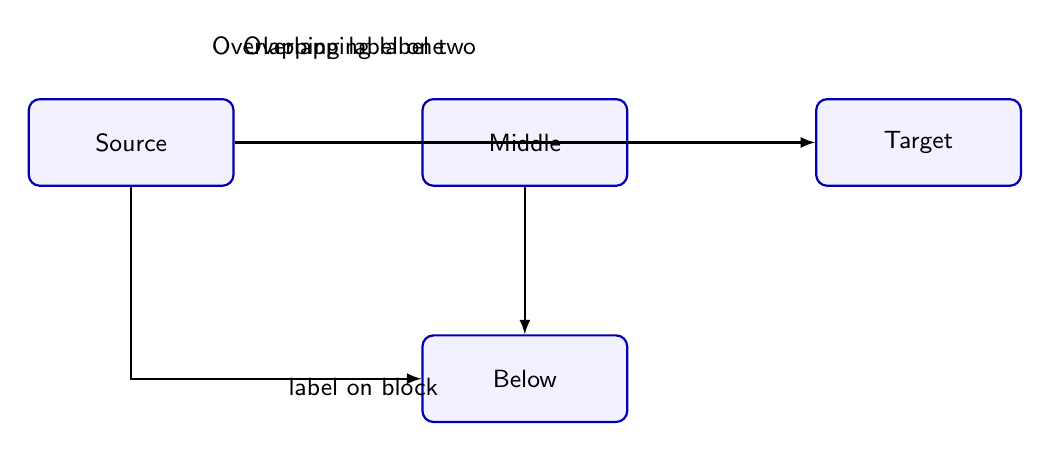
\begin{tikzpicture}[>=latex, font=\sffamily\small]
  \tikzstyle{blk} = [draw=blue!70!black, fill=blue!5, thick, rounded corners,
                     minimum width=2.6cm, minimum height=1.1cm, align=center]

  \node[blk] (a) at (0,0)   {Source};
  \node[blk] (mid) at (5,0) {Middle};
  \node[blk] (b) at (10,0)  {Target};
  \node[blk] (c) at (5,-3)  {Below};

  % LOI 1: mui ten tu a sang b di THANG XUYEN QUA block "mid"
  \draw[->, thick] (a.east) -- (b.west);

  % LOI 2: hai nhan de len nhau
  \node[text=black] at (2.5,1.2) {Overlapping label one};
  \node[text=black] at (2.9,1.2) {Overlapping label two};

  % LOI 3: nhan de len block "c"
  \draw[->, thick] (a.south) |- (c.west) node[pos=0.9, above=-0.35cm] {label on block};

  % canh hop le de kiem tra khong bao sai
  \draw[->, thick] (mid.south) -- (c.north);
\end{tikzpicture}
\end{document}
